
	This chapter describes implementation details about the developed control methods described in the previous chapter \ref{chapter:Proposed Interface System}.

\section{Application architecture}

	For the interaction with the iCub through the Kinect and the \ac{Wiimote}, several modules were developed. All the software developed throughout this work, was made using the C++ language, the Yarp libraries and, the iCub libraries. Some of the modules created were used just for data visualization and comprehension. Next we will describe the main modules created for the \ac{Wiimote} and the Kinect interaction interaction with the iCub, the data vizualization modules developed are not described because they were only used for development support.
	
	\ac{Yarp} makes it possible to run modules in different machines and networks, connecting them through the port abstraction. This allows a separation between the modules that interface with the devices, the modules that work on converting the devices data into interaction commands, and the control modules for the iCub, the two devices considered are the \ac{Wiimote} and the Kinect.

	\begin{figure}[htb]
	\begin{center}
	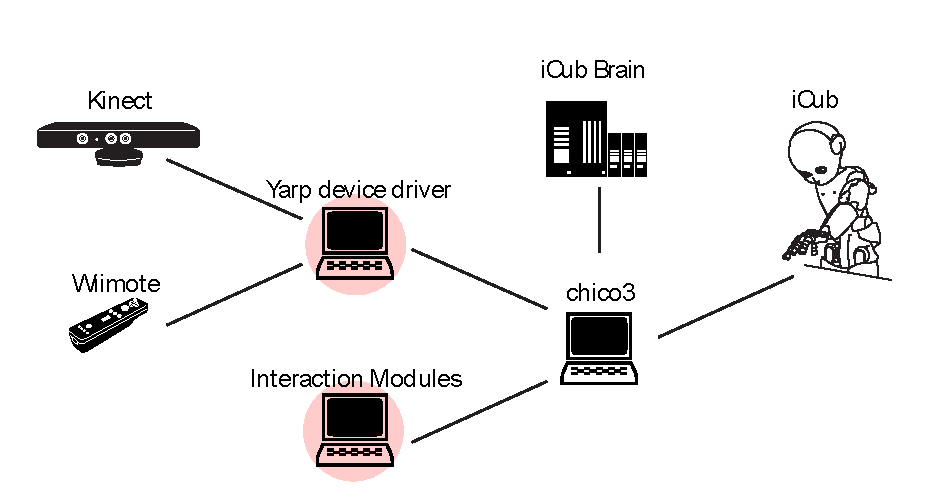
\includegraphics[width=120mm,page=1,angle=0]{icubSimpleNetworkDiagramMafalda-crop.pdf}
	\end{center}
	\caption[iCub Network Diagram]{Kinect/\ac{Wiimote} Yarp drivers and iCub network diagram.} 
	\label{fig:iCubNetDiagram}
	\end{figure}

	The figure \ref{fig:iCubNetDiagram} is a representation of the network of modules created and used, and how they relate to other machines.
	
	The Yarp device drivers are the device interfaces created. More specifically they are two distinct modules (one for the \ac{Wiimote} another for the Kinect) that are recursively retrieving data from the Kinect and the \ac{Wiimote}, and redirecting that data in a usable format to the output ports specified in a initialization file. These modules also have input ports that are used for the remote alteration of the device settings, such as activation of actuators, or the internal state reset.
	
	The interaction modules, respond to events that occur on ports connected to the Yarp device driver ports, and output using the iCub libraries to the iCub ports. The events consist of data captured by the interaction device and sent to a port, this data is converted into motor angle values or Cartesian point values by the interaction modules that are interpreted by the iCub library functions.
	
	Chico3 is a laptop computer where the the Yarp Server normally runs, and where typically the iCub modules are called to be executed on remote machines, such as the iCubInterface in the PC104 computer mounted in the iCub or the iKin Solver/Controller modules in the iCubBrain server.
	
	Every module developed respects the Model-View-Controller architecture:
\begin{description}
\item[Model] this concept is present in all modules. In the device driver it is responsible for the interaction device data streaming, and in the interaction control modules it is responsible for the conversion between interaction data and motor angles, or useful Cartesian points.
\item[View] this concept is present in all the modules. In the device driver it is in the form of the interaction device, used to interface with the user. In the interaction control modules it is present as the results outputted to the iCub robot, the result from the interaction.
\item[Controller] this concept is present in all modules. It is the concept responsible for the port and data management, in both, interaction control module and device driver.
\end{description}

	There was a concern through out the work to make every class implemented reusable, and understandable, to whomever might want to run or reproduce it.

\section{Main libraries used}
	
	The Yarp and iCub come with C++ libraries for developers to use. The libraries permit coding abstracted from the technical details of the devices and encoders and focus on control and communication issues.
	
	Both of these libraries were fundamental for the \ac{Wiimote} and Kinect modules development. These libraries are the ones that allow to control the iCub and to set up a simple distributed solution.
	
\subsection{Yarp}

	To remotely send instructions and retrieve the status from encoders and devices there is a Yarp server continuously running, this server maintains a list of ports that are available. When a connection is made to one of the ports available Yarp connects, directly without the data passing through the network node that is running Yarp, to the network node that created the port. Typically each program creates its own ports and connections are made port to port, each program is only responsible for maintaining its own ports, this avoids Yarp server from becoming a bottleneck managing several connections. The ports created are \ac{TCP} ports that abstract the data passed from the network node specific characteristics. Using the \ac{Yarp} ports it is possible to get a distributed solution to work with the devices that connect through a Yarp network.

	To communicate to a specific device it is good practice to create a specific Yarp device driver, these device drivers are to a user always instantiated in the same way and return a interface object that has a set of functions specific to interface with that device. Usually each device needs some program to be running to get or set the values of the device directly. The program that uses the device is the one responsible for the management of the Yarp ports, this management involves keeping the ports alive and using the ports to respond to calls made by other programs that might be using the device. Through the ports it is possible to get media, text, or numeric data.
	
	In the Yarp repository there are already many different drivers available that can be used, but a programmer can also create a new driver from scratch, as the Kinect and \ac{Wiimote} were. The drivers created are accompanied by a program that controls the device directly. The drivers mostly abstract the users from the ports by using the functions available in the driver interface class, with drivers the communication is still made through the Yarp ports. Although abstracted the suggested architecture to be implement by the program interfacing with the device is divided into two main classes, a Port Thread class that is responsible for setting up ports and is constantly updating, and a Device Driver class that interfaces with the device while it calls or it is being called by the Port Thread class. The Port Thread class has two base classes \texttt{RFModule} and \texttt{TypedReaderCallback}. The \texttt{RFModule} is a helper class that has already implemented a thread and needs that the virtual methods for updating and configuring the thread to be implemented. The \texttt{TypedReaderCallback} is a callback class that is passed to a port, as an object, and for each port event it calls a virtual method to be defined by the user. A simple representation of the Yarp device driver main classes is shown in figure \ref{fig:YarpDeviceDriverSimpleRepresentation}
		
	\begin{figure}[htb]
	\begin{center}
	\includegraphics[scale=0.30,page=4,angle=90]{icubSimpleNetworkDiagram-crop.pdf}
	\end{center}
	\caption[Simple representation of Yarp Device Driver main classes]{Simple representation of Yarp Device Driver main classes.} 
	\label{fig:YarpDeviceDriverSimpleRepresentation}
	\end{figure}
	
	Yarp is described as being the pipes in a water system\footnote{\url{http://eris.liralab.it/yarpdoc/what_is_yarp.html}}. Yarp itself can be used for many purposes other than robotics, it sets up a way for different programs to communicate with each other over a \ac{TCP} network. This becomes very useful for intense processing tasks that need to be distributed through several computers. The libraries available with Yarp can even abstract programmers more from the communication ports that Yarp uses allowing to call functions remotely as they were part of the programs library, using the Yarp ports underneath. Yarp server although needed so that ports can connect to each other is only used as a port listing service, the connected ports communicate directly through \ac{TCP} and if the communication is made through the same computer the communication is made without the \ac{TCP} by memory access. By splitting the device driver from the robot controller the modules developed take advantage of the Yarp framework. The robot controller drivers follow some of the ideas implemented in the Yarp device driver, such as the use of a Port Thread class, although it has many characteristics that are discussed in the next chapter because they are iCub specific. 

\subsection{iCub}
	
	In the iCub, repository there can be found not only code contributions of different projects done with the robot, but also a library that is used with Yarp implementing drivers and useful utilities.
	
	In this repository is a critical program called iCubInterface. The iCubInterface initializes all the motors in the robot, and sets up all the ports that are used to control the motors. The iCubInterface is the program that setups the ports for the motorboard driver, which is a generic driver from Yarp, for interfacing with the motors. This program directly uses the motors setting and getting their encoder status. The iCubInterface is generic enough to be adapted to robots other than the iCub, such as it was done with the Vizzy robot. The adaption is done by altering an initialization file, that specifies which motors connect to which port, more than one motor is reached through a single port, although each motor is only connected to one port. For each port prefix there are three ports set, a status port, a command port, and a \ac{RPC} port. The status port indicates the status of the motors, the command port receives commands, and the \ac{RPC} port receives \ac{RPC} calls and acknowloges them. The port prefixes setup for the icub are:

	\begin{verbatim}
		/icub/head
		/icub/face
		/icub/cam
		/icub/torso
		/icub/righ_arm
		/icub/left_arm
		/icub/right_leg
		/icub/left_leg
	\end{verbatim}

	The names of the ports are self explanatory, each one controlling a set of joints, with the exception of the \verb\/icub/face\ and \verb\/icub/cam\, where one is connected to the facial expressions of the iCub, and the other is connected to the iCub cameras respectively. Both \verb\/icub/face\ and \verb\/icub/cam\ are not the typical prefixes, not having the three ports for status, command, and \ac{RPC}, but the face has eyelids, and the cameras are left or right, with fovea and logpolar ports.
	
	The motorboard driver can control the motors in two distinct forms, either by position or by velocity. The position control is made by specifying the motor angle that a user wants to reach, the driver maintains a internal state of the angle changes that is read from the encoder. When a new angle is determined, and a reference speed and acceleration has been chosen, the motor moves according to these values to the specified position. The velocity control is done by specifying the speed which a user wants a motor to move, positive velocities move in a positive direction, negative ones move in a negative direction, also here a reference acceleration needs to be specified. These control forms are instantiated by two classes which interface through the iCubInterface ports, the \texttt{IPositionControl} and \texttt{IVelocityControl}.
	
	In the motor interaction controller modules developed, only the velocity control was used, this choice was made because a better control could be made. The applications send timed updates of the control values to the motors, when the position control was used the response time was higher resulting in sometimes unpredictable movements, particularly noticeable in the case of the Vizzy robot, that also used the ICubInterface, the motor made a unpleasant clicking sound whenever a new position value interrupted an already moving motor. With the velocity control the speed defined depended on the current angle and on the desired angle, that was maintained internally to the program calling the velocity control, if the difference between the desired and current angle was negative it meant a negative movement should be made and vice-versa. Also the speed chosen depended on how far the current angle and the desired angle were, the closer they were the lower the velocity was, this avoided a wobbling effect that happened when using the position control.
	
	Another driver available is the iKin, the iKin has a set of functions that facilitate the use of the inverse kinematics of the iCub. Like the iCubInterface, this driver is generic enough to be adapted to the Vizzy robot by rewriting a initialization file with the kinematic chain specified in the Denavit-Hartenberg convention. There are two programs that accompany the iKin driver, a solver and a controller. The programs are not merged into a single one, because besides separating robot control from the kinematics control, they are very process intensive, this way they can be run in different computers through the Yarp ports. The iKin solver receives the current status of the motors that it needs to move and calculates the positions to which the motors need to move so that the end-effector can reach, or try to reach, a point given in Cartesian coordinates, this is where the inverse kinematics are calculated. The iKin controller defines the velocities and acceleration that each motor should be set to, while moving to a angle, the goal is to make the iCub do a more natural, and human like, movement. When using the iKin driver the iKin solver and controller need to be running simultaneous because they exchange messages between them, so that the controller and the solver know what are the angles desired for the iCub motors. The driver also permits to set characteristics for this type of control as the tolerance to consider a desired end-effector target achieved, or the amount of time to go from current end-effector pose to the desired end-effector pose.
	
	The kinematic modules use the \texttt{ICartesianControl} class, the \texttt{goToPosition()} function can be called with or without a orientation defined, in the implemented modules case, it was decided that the orientation would only be defined when controlling solely the orientation, so only the \ac{Wiimote} kinematic control module uses the orientation in one of its modes. This was decided because when trying to reach a point with the Cartesian control if the orientation was defined, the Cartesian Solver module would have to weight between reaching the point and having the correct orientation, and to our goal it was more interesting reaching the desired point in the best way possible. The speed of the movement made can be defined by the amount of time that it will take to reach from the current pose to the desired pose, this time is set in the initialization file, so a small movement by the user will result in a slow movement by the robot and a large movement by the user will result in a faster movement by the robot.
	
	The suggested implementation of the interaction control modules, use both the position control and kinematic control to interact with the iCub robot, although the interaction methods differ, all the modules have a similar class diagram. As in the Yarp Device Driver there is a Port Thread class that sends, and receives data from the Yarp device driver, and also calls functions from an abstract class that controls the iCub robot the \verb\iCubGeneric\ class, the Port Thread also uses as base classes the \texttt{RFModule} and \texttt{TypedReaderCallback} classes as in the previously described module. The \verb\iCubGeneric\ abstract class as virtual functions that must be implemented by the classes that inherit from it, and simple functions and data structures that maintain the needed data to control the robot. The virtual functions that must be implemented, initialize the robot, close the robot connection, and update the robot. It was chosen that the \verb\iCubGeneric\ maintained its own internal state data from the interaction device, because it allowed to separate the update rate of the robot and the device data update rate, so a event in a data port does not mean an immediate reaction of the robot state, this makes time for a better control of the robot, the need to send commands to the robot is much less frequent than the data updates from the interaction devices. The classes that implement the \verb\iCubGeneric\ class control the robot either through the kinematic control or the motor control, this inheritance was useful because the Port Thread never cares about how the robot is controlled, but it cares about at what rate must the robot state be updated, when does it start, or stop controlling the robot, and what data should be passed on to the robot. Conversion of the data into useful movements is done by two classes that are implementations of the \verb\iCubGeneric\ class, one specific for the kinematic control, another for the motor control, these are the classes that have to be implemented depending on how it is supposed for the iCub to interpret the device data, they both implement all the virtual methods from the \verb\iCubGeneric\. A simple representation of the explained interaction module can be seen in figure \ref{fig:InteractionModuleSimpleRepresentation}.
	
	\begin{figure}[htb]
	\begin{center}
	\includegraphics[scale=0.30,page=5,angle=90]{icubSimpleNetworkDiagram-crop.pdf}
	\end{center}
	\caption[Simple representation of the Interaction Module main classes]{Simple representation of Interaction Module main classes.} 
	\label{fig:InteractionModuleSimpleRepresentation}
	\end{figure}
	
	The iCub libraries available allow to connect to the iCub and its devices as a normal device driver, abstracting the programmer from all the specific iCub control issues. The motor access is done through the \verb|remote_controlboard| driver by using the iCubInterface, which is responsible for maintaining the ports that interface with the robot motors. The iCub library has a kinematic control driver, the iKin, that allows the inverse kinematic control of the iCub. Because the iKin task is a heavy processing task, it is divided into two programs a controller and a solver, these programs not only solve the kinematic task, but try to achieve a natural movement by defining the motor speeds depending on the movement to be done. The interaction modules developed separate the data retrieval from the robot motors update without the port control block and the robot control block having a high dependency on each other, this made possible a independent implementation and tweaking of the control from the data retrieval. Also the implementation suggested keeps the update rates separated making a more convenient control available, where a control instruction can be sent after analyzing several device data updates, which come at a much higher rate than the needed for the robot control.

\section{Wiimote modules}

	The \ac{Wiimote} iCub controller application is divided into three modules ,as can be seen in figure \ref{fig:WiimoteNetworkDiagram}, the \ac{Wiimote} Yarp driver (device driver), the \ac{Wiimote} solver, and the Robot controller (interaction controller). Each of these modules is a independent program that might be run on a different computer, connected through the Yarp network. The \ac{Wiimote} Yarp driver and the \ac{Wiimote} Robot Controller follow the architecture defined before, although they solve specific problems of the \ac{Wiimote} interaction and device interface.
	
	\begin{figure}[htb]
	\begin{center}
	\includegraphics[scale=0.50,page=2,angle=90]{icubSimpleNetworkDiagram-crop.pdf}
	\end{center}
	\caption[\ac{Wiimote} modules diagram]{\ac{Wiimote} Yarp modules and iCub controller.} 
	\label{fig:WiimoteNetworkDiagram}
	\end{figure}
	
	The \ac{Wiimote} Yarp driver module is the interface between the \ac{Wiimote} device and the Yarp Network. The library chosen to interface with the \ac{Wiimote} and the \ac{MP} extension was the wiiuse\footnote{\url{http://sourceforge.net/projects/wiiuse/}} library that comes with the fwiineur\footnote{\url{http://fwiineur.blogspot.com/search/label/release}} libraries. The fwiineur is a set of libraries that allow MATLAB and SCILAB to acquire data from the \ac{Wiimote} device, the wiiuse library used by the fwiineur was altered to get data from the \ac{MP} extension, the original wiiuse does not have this feature implemented although it can be programmed to do this by reading the data from the proper \ac{Wiimote} memory address, and interpreting that data.
	
	In the Wiimote Module there is a initialization file where all the port names prefix, velocities and robot name are set. The module starts by opening five ports, from which the prefix is specified in a initialization file, by default the prefix is \verb\/wiimote\. The ports opened are:
	
	\begin{verbatim}
	/wiimote[NUMBER]/sensor
	/wiimote[NUMBER]/ext/mp 
	/wiimote[NUMBER]/status 
	/wiimote[NUMBER]/reader
	/wiimote[NUMBER]/bots
	\end{verbatim}
	 
	Because there can be up to four \acp{Wiimote} connected simultaneously, all the excess ones are ignored, the port prefix \verb\/wiimote[NUMBER]\ has a number indicating the \acp{Wiimote} ID. All the ports are output ports, that send data whenever the main thread is updated, with the exception of the \verb\/wiimote[NUMBER]/reader\ port, that is a reading port which allows to set the \ac{Wiimote} sensors and actuators, on and off.
	
	The \verb\/wiimote[NUMBER]/sensor\ outputs the sensor values, per each set of values a vocab is written before. Each of the sensors needs to be turned on, which is done when a command is received in the reader port indicating what sensor should be turned on or off. The \ac{IR} camera value is preceded by the \verb|[IR]| vocab, and sends up to four Cartesian points to the sensor port, representing each of the \ac{IR} sources. The accelerometer value is preceded by the \verb|[ACC]| vocab, and outputs a vector that is defined by the accelerometer position relatively to gravity.
	
	The \ac{Wiimote} solver module connects to the \verb\/wiimote[NUMBER]/ext/mp\ port, which sends data from the \ac{MP} extension, and on each read event, updates a internal rotation matrix. In this module there is a reader port that can receive a new rotation matrix to overwrite the current one. This matrix represents all the rotations made with the \ac{Wiimote} in the form \begin{math}R_{x}R_{z}R_{y}\end{math}. This module outputs its internal rotation matrix, and the vector \texttt{(0,1,0)} rotated by the rotation matrix. When the \ac{MP} extension is turned on there is a calibration process where the average of noise output by the gyroscope is calculated and removed from the values acquired, only after this calibration, which needs the \ac{Wiimote} to be on a stable position for a moment, the \verb\/wiimote[NUMBER]/ext/mp\ port starts outputting data.
	
	The \ac{Wiimote} Robot controller module connects to the ports opened by the solver module and the Yarp driver module. This module uses the iCub library to connect to the robot ports through the \verb\PolyDriver\ interface. This interface abstracts the iCub control through simple functions that make all the needed port connections and send all the important data. It is possible to control the robot upper part by directly calling the motor joints, and defining a velocity, acceleration and angle, or by using a the iKin library that abstracts the kinematic control of the robot to a Cartesian point of the end-effector, the details of these module were described in the previous section.
	
\section{Kinect modules} 

	The Kinect iCub control application is divided into two modules as can be seen in figure \ref{fig:KinectNetworkDiagram}, the Kinectic Yarp driver (device driver), and the Kinect robot controller (interaction controller). Each of these modules is a independent program that might be run on a different computer, connected through the Yarp network. The \ac{Wiimote} Yarp driver is also used because the B button on the remote is used as a on/off switch for the interaction. The Kinect Yarp driver and the Kinect Robot Controller follow the architecture defined before, although they solve specific problems of the Kinect interaction and device interface.
	
	\begin{figure}[htb]
	\begin{center}
	\includegraphics[scale=0.50,page=3,angle=90]{icubSimpleNetworkDiagram-crop.pdf}
	\end{center}
	\caption[Kinect modules diagram]{Kinect Yarp modules and iCub controller.} 
	\label{fig:KinectNetworkDiagram}
	\end{figure}
	
	The Kinect Yarp driver module is the interface between the Kinect interaction device and the Yarp network. To interface with the Kinect sensor the OpenNi/NITE library was used. The OpenNi/NITE was created by PrimeSense, OpenNI is a generic library to connect to a broad set of devices, NITE is used by the OpenNI to interface directly with the Kinect device. Although there was already a Kinect driver in the Yarp repository, it did  not made the tracking of the skeleton, because the libfreenect library that was used did not have the skeleton tracking algorithm implemented yet, so using the OpenNi/NITE library was preferred. This module can make two types of tracking, skeleton and hand tracking, the type of tracking desired is specified in the initialization file, only one output port is opened, there was no need for input ports because no settings needed to be changed on the Kinect for the interaction to work. During the skeleton tracking at each update of the Port Thread a set of ordered Cartesian points and rotation matrices, that describe the kinematic skeleton of a person detected by the Kinect sensor, is output to a port. The description of the skeleton is made in two forms, a set of points in the Cartesian space, and a set of rotation matrices that are indexed to each of the skeleton joints, also there is a confidence value for each element (matrix or Cartesian point) that indicates how accurate the element is. The hand tracking only outputs two values at each update, a Cartesian point and a confidence value.
	
	The Kinect Robot controller module connects to the port opened by the Kinect Yarp driver module, and updates its internal state data on each port event, sending commands to the robot at a different rate. In the initialization file it can be specified what is the desired type of control, motor control for the skeleton tracking or the kinematic control for the hand tracking, depending on the desired tracking it is expected that the port messages come in a specific format. The data received from the Yarp driver port, while tracking the skeleton, in the form of rotation matrices, is factored as \begin{math}R_{x}R_{y}R_{z}\end{math} and mapped into three motor angles. The rate at which the skeleton values are updated and at which the robot control is done are different, because it was better to maintain a smoother control without respecting the Kinect frame rate. The robot controller uses the \verb|remote_controlboard| iCub driver move the motors independently to the desired angles. While the robot controller module is tracking the hand the Cartesian point read from the port is mapped to the \verb|cartesiancontrollerclient| device end-effector for the robot. This module only takes into account the first user detected ignoring all the others.
	
\section{Concluding remarks}

	In this chapter the applications developed for interface with the iCub robot were described.
	
	Both the applications followed a similar structure, the abstraction was made on several levels so that it could be easily reused by other projects.
	
	Of the \ac{Yarp} framework was taken advantage to separate the interface device drivers from the interaction controller logic of the robot. In the case of the \ac{Wiimote} module a specific application was created to handle the angular movement status, which might be replace by other application if needed with out needing to change either the control application or the driver application.
	
	Both of the driver application created were actually in another robot besides the iCub, the Vizzy robot, the Kinect driver was used during several presentations. To achieve the desired effect it took less than a week, and no changes were required in either of the drivers, only motor mapping needed to be readjust to map the correct motors joints in the most proper way.
